\documentclass{ujarticle}
\renewcommand{\baselinestretch}{0.85}
\usepackage[top=1.5cm, bottom=1.5cm, left=1.5cm, right=1.5cm]{geometry}
\usepackage{xcolor}
\usepackage[dvipdfmx]{graphicx, hyperref}

% \usepackage{subfig}
\usepackage{url}
\usepackage{stackengine}
\usepackage{multirow}
\usepackage[hang,small,bf]{caption}
\usepackage[subrefformat=parens]{subcaption}
\captionsetup{compatibility=false}

\newcommand{\Sref}[1]{\mbox{\ref{sec:#1}}}
\newcommand{\Tref}[1]{\mbox{表\ref{tab:#1}}}
\newcommand{\Eref}[1]{\mbox{式(\ref{eq:#1})}}
\newcommand{\Fref}[1]{\mbox{図\ref{fig:#1}}}

\captionsetup[subfigure]{labelformat=simple}
\renewcommand{\thesubfigure}{(\alph{subfigure})}

\hypersetup{
	setpagesize=false,
	bookmarksnumbered=true,
	bookmarksopen=true,
	colorlinks=true,
	linkcolor=black,
	citecolor=black
}

\begin{document}
    \begin{flushright}
        MDLab GM資料\\
        22年11月1日(火)
    \end{flushright}

    \begin{center}
        {\Large	距離学習を導入したCenterNetによる\\腹部超音波画像からの肝腫瘍検出と分類}
    \end{center}

    \begin{flushright}
        {\large B4 原 英吾}\\
    \end{flushright}

    \section{研究背景および目的}
        \begin{itemize}
            \item 背景
            \begin{itemize}
                \item 器具の操作と診断を同時に行わなければならず高難易度
                \begin{itemize}
                    \item 特に悪性腫瘍(肝細胞がんと転移性肝がん)は見逃してはならない
                \end{itemize}
                \item 先行研究
                \begin{itemize}
                    \item 2段階の推論ステップを踏んでいる4クラス検出を行う
                    \item 精度は0.7617($\approx 0.8550 \times 0.8909$)
                    \begin{itemize}
                        \item YOLOv5での検出(Recall): 0.8550
                        \item VGG16での分類(Accuracy): 0.8909
                    \end{itemize}
                    \item 円形である腫瘍の検出に適していない可能性がある
                    \begin{itemize}
                        \item YOLO系統は様々なアスペクト比の物体を検出するという前提のモデル
                    \end{itemize}
                    \item 大域特徴を用いないで分類するため精度が落ちている可能性がある
                    \begin{itemize}
                        \item 腫瘍領域として切り取られた診断画像に対して分類をしている
                    \end{itemize}
                \end{itemize}
            \end{itemize}
            \item 目的
            \begin{itemize}
                \item 既存の研究を踏まえたモデルの精度向上
                \begin{itemize}
                    \item 単一モデルで推論を行うことで精度向上を目指す
                \end{itemize}
                \item 超音波支援システムの開発
            \end{itemize}
        \end{itemize}

    \section{これまでの研究のまとめ}
        \begin{figure}[!b]
            \begin{minipage}[t]{0.627\linewidth}
                \centering
                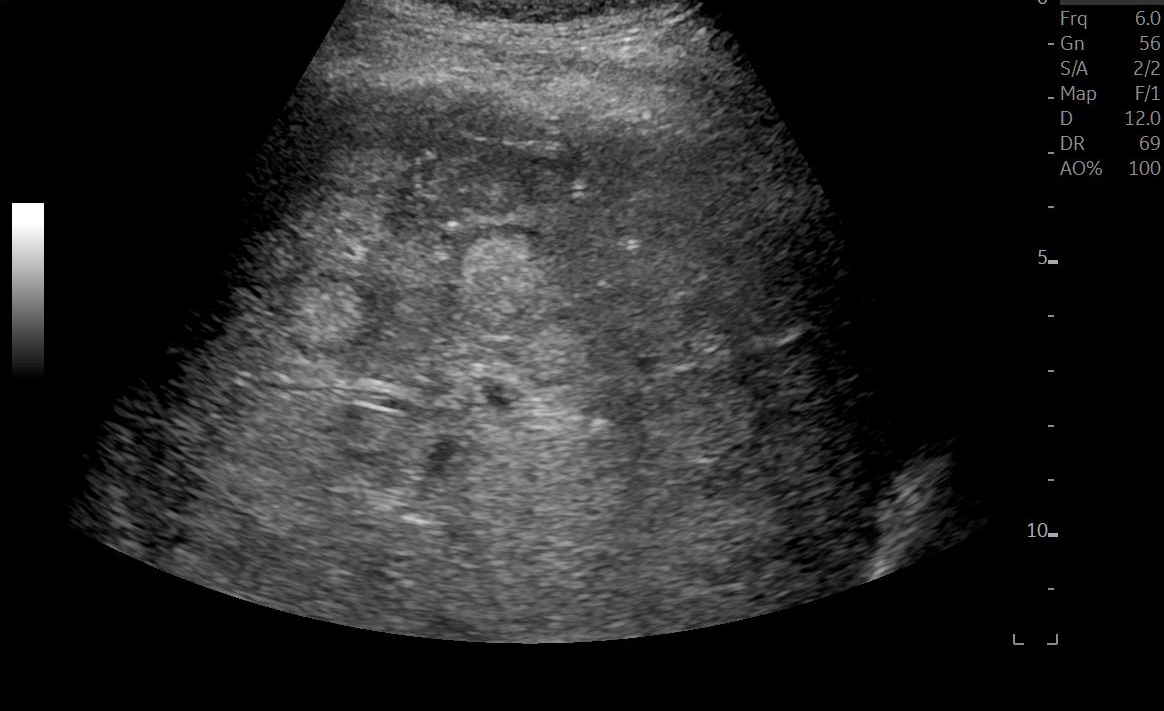
\includegraphics[width=\linewidth]{../fig/us.png}
                \subcaption{データセット内の診断画像(ラベル不足あり)}
                \label{fig:us}
            \end{minipage}
            \begin{minipage}[b]{0.366\linewidth}
                \centering
                \subfloat[単純嚢胞]{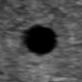
\includegraphics[width=.48\linewidth]{../fig/cyst.png} \label{fig:cyst}}
                \subfloat[血管腫]{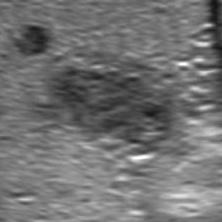
\includegraphics[width=.48\linewidth]{../fig/hemangioma.png} \label{fig:hemangioma}}

                \subfloat[肝細胞がん]{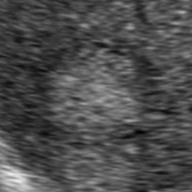
\includegraphics[width=.48\linewidth]{../fig/hcc.png} \label{fig:hcc}}
                \subfloat[転移性肝がん]{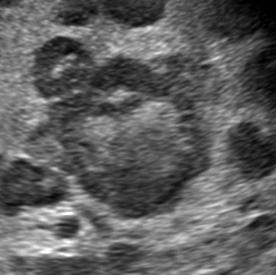
\includegraphics[width=.48\linewidth]{../fig/meta.png} \label{fig:meta}}
            \end{minipage}
            \caption{実験で用いる超音波画像例}
            \label{fig:ex}
        \end{figure}

        \begin{itemize}
            \item データセット
            \begin{itemize}
                \item 国立研究開発法人日本医療研究開発機構(AMED)\footnote{\url{https://www.amed.go.jp/}}から提供された延べ8万枚のデータ
                \begin{itemize}
                    \item 腹部超音波画像,ROI,年齢,性別,撮影器具など
                \end{itemize}
                \item \Tref{dataset}で示す様にtrain : validation : test = 8 : 1 : 1に分割する
            \end{itemize}
        \end{itemize}
        \begin{itemize}
            \item 実験手順
            \begin{enumerate}
                \item SimSiamでbackboneを事前に距離学習させる
                \item CenterNetで学習
                \begin{itemize}
                    \item 距離学習させたバックボーンネットワークの重みを有効活用するために層単位で段階的に解除していく
                \end{itemize}
                \item CenterNetのみで推論
                \begin{itemize}
                    \item 信頼度のしきい値はF1値が最大となる時の値
                \end{itemize}
            \end{enumerate}

            \begin{table}[t]
                \centering
                \caption{データセット分割後のそれぞれの枚数}
                \label{tab:dataset}
                    \begin{tabular}{l|rcr|c} \hline
                        \multicolumn{1}{c|}{診断名} & \multicolumn{1}{c}{train} & validation & \multicolumn{1}{c|}{test} & 合計 \\ \hline
                        単純嚢胞 & 24,217 & 3,018 & 3,037 & 30,272 \\
                        血管腫 & 23,749 & 3,059 & 2,962 & 29,770 \\
                        肝細胞がん & 10,934 & 1,310 & 1,371 & 13,615 \\
                        転移性肝がん & 8,222 & 1,003 & 1,021 & 10,246 \\ \hline
                        合計 & 67,122 & 8,390 & 8,391 & 83,903 \\ \hline
                    \end{tabular}
            \end{table}
        \end{itemize}

        \begin{itemize}
            \item 結果
            \begin{itemize}
                \item 分類精度が向上
                \begin{itemize}
                    \item 大域特徴を用いて分類することができた
                    \item SimSiamによる影響も大きそう
                \end{itemize}
                \item 検出精度は向上していない
                \begin{itemize}
                    \item 距離学習で検出に不向きな特徴量を学習してしまった
                    \item 検出のheadを分離する?
                \end{itemize}
                \item エッジデバイスでの使用が易化
                \begin{itemize}
                    \item 推論必要なメモリメモリが50\%に
                    \item 推論スピードが33\%に
                \end{itemize}
            \end{itemize}
        \end{itemize}

        \begin{table}[!h]
            \centering
            \caption{提案手法を用いたモデルでの評価指標毎の値}
            \label{tab:metric}
                \begin{tabular}{lr|rr|ccc|rr|ccc} \hline
                    & & \multicolumn{5}{c|}{提案手法} & \multicolumn{5}{c}{YOLOX} \\
                    診断名 & \multicolumn{1}{c|}{腫瘍数} & \multicolumn{1}{c}{FP} & \multicolumn{1}{c|}{FN} & Precision & Recall & F1 & \multicolumn{1}{c}{FP} & \multicolumn{1}{c|}{FN} & Precision & Recall & F1 \\ \hline
                    Cyst & 3,037 & 492 & 357 & 0.832 & 0.873 & 0.852 & 851 & 297 & 0.741 & 0.892 & 0.809 \\
                    HCC & 1,371 & 168 & 339 & 0.722 & 0.601 & 0.657 & 371 & 371 & 0.471 & 0.591 & 0.524 \\
                    Hem. & 398 & 301 & 465 & 0.828 & 0.796 & 0.812 & 468 & 591 & 0.740 & 0.744 & 0.742 \\
                    Meta & 1,021 & 172 & 290 & 0.619 & 0.543 & 0.578 & 28 & 339 & 0.686 & 0.106 & 0.183 \\ \hline
                    合計 & 8,391 & 1,133 & 1,451 & 0.750 & 0.703 & 0.725 & 1,718 & 1,598 & 0.685 & 0.695 & 0.690 \\ \hline
                \end{tabular}
        \end{table}

        \begin{table}[!h]
            \centering
            \caption{従来手法,YOLOXと提案手法の比較}
            \label{tab:comparison}
            \resizebox{\width}{!}{
                \begin{tabular}{l|rr|rrr|r} \hline
                    & 使用メモリ(MB) & 推論速度(/sec)& 再現率$_{det}$ & 精度$_{cls}$ & \multicolumn{1}{c|}{4クラス検出精度} & \multicolumn{1}{c}{信頼度} \\ \hline
                    \multicolumn{1}{c|}{従来手法\cite{yamagishi2022detection,nishida2022artificial}} & 3898.3 & 0.0272 & 0.8550 & 0.8909 & 0.7617 & 0.30 \\
                    YOLOX\cite{ge2021yolox} & 4178.9 & 0.0167 & 0.8096 & 0.8447 & 0.6839 & 0.35 \\
                    \textbf{提案手法} & \textbf{1838.2} & \textbf{0.0095} & \textbf{0.8271} & \textbf{0.9206} & \textbf{0.7614} & \textbf{0.40} \\ \hline
                \end{tabular}
            }
        \end{table}

\clearpage

    \section{前回GMからの進捗}
        \begin{itemize}
            \item UMAPを用いて可視化
            \begin{itemize}
                \item \Fref{umap_before}は散らばってしまっているので初期の重みとしては不適切
            \end{itemize}
            \item WiNFの原稿を書いて申し込んだ(先生方ありがとうございました)
        \end{itemize}

        \begin{figure}[!h]
            \centering
            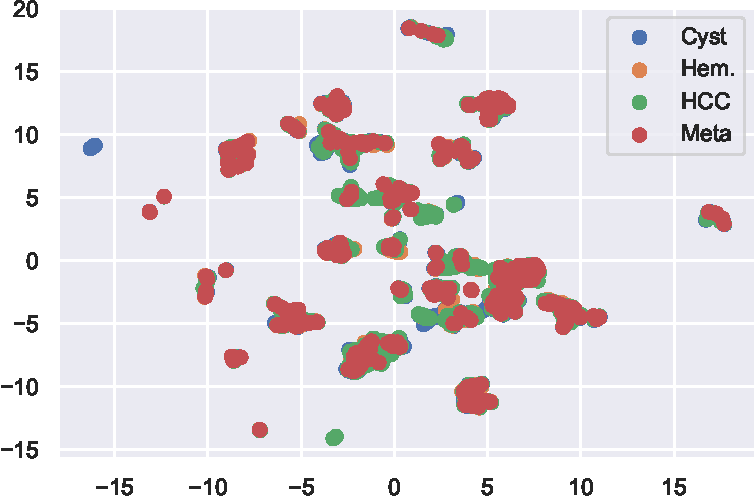
\includegraphics[]{../fig/umap_before}
            \caption{ImageNetで事前学習済みのResNet18を用いた可視化}
            \label{fig:umap_before}
        \end{figure}

    \section{今後の課題\&スケジュール}
        \begin{itemize}
            \item 11/15までに
            \begin{itemize}
                \item SimSiamで学習済みのResNet18を用いてUMAPで可視化したい
            \end{itemize}
            \item 12/1までに
            \begin{itemize}
                \item IWAIT2023の原稿提出期限
            \end{itemize}
            \item 12/17までに
            \begin{itemize}
                \item WiNF2022の発表スライド?
            \end{itemize}
            \item 12/20までに
            \begin{itemize}
                \item 卒論の原稿(粗めでも可)
            \end{itemize}
            \item 1/8までに
            \begin{itemize}
                \item IWAIT2023の発表スライド?
            \end{itemize}
        \end{itemize}

    \bibliographystyle{../spiebib}
    \bibliography{../paperlist}
\end{document}
